\documentclass[12pt]{article}
\usepackage{geometry}                % See geometry.pdf to learn the layout options. There are lots.
\geometry{letterpaper}                   % ... or a4paper or a5paper or ... 
\usepackage[parfill]{parskip}    % Activate to begin paragraphs with an empty line rather than an indent
\usepackage{graphicx}
\usepackage{amssymb, amsmath}
\usepackage{fullpage}

\usepackage{fourier}
\usepackage{courier}

\setcounter{secnumdepth}{0} % supresss section numbers

% Nice captions.
\usepackage[hang,small,bf]{caption}
\setlength{\captionmargin}{25pt}

\title{Aggregation Optimizations for Skewed Data}
\author{Josh Rosen}

\begin{document}
\maketitle

\section{Introduction}

Aggregate-by-key is a common (and often expensive) operation in ``big data''
frameworks like MapReduce and Spark.
%
There are many ways to optimize aggregation, including multi-level
aggregation techniques, like aggregation trees, and pre-aggregation
techniques, like Hadoop and Spark's map-side combiners.

As a framework for analyzing these optimizations, we can view aggregators as
functions whose output key distributions are ``flattened'' versions of their
input key distributions.  The degree of this flattening depends on the aggregation
technique and properties of the input data, such as clusteredness or skew.

For example, a buffering aggregator with unlimited buffer space produces
uniform output key distribution for any input distribution.  A pre-aggregator
with finite buffer space may leave the key distribution untouched in the worst
case, or may achieve perfect flattening in the best case.

\subsection{Analysis Framework}

In our framework, an aggregator is a stateful operator that receives an input
stream of (key, value) pairs and produces an output stream of (key, aggregate)
pairs.  Let each input key $k$ be randomly sampled with replacement
from a discrete distribution $p_{in}(k)$.  The aggregator's behavior defines
a distribution of output sizes and output key distributions $p_{out}(k)$.
The output key distribution is guaranteed to be at least as uniform as the
input distribution.

\begin{figure}
\begin{center}
    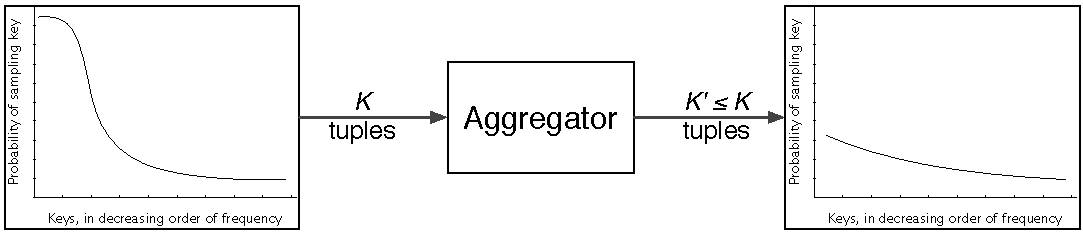
\includegraphics[width=\textwidth]{figures/aggregator_as_filter}
\end{center}
\caption{Aggregators can be viewed as stream filters that perform lossless
compression by removing skew.}
\label{fig:aggregator_as_filter}
\end{figure}

As an example, an aggregator with unlimited buffer space produces output whose
size is equal to the number of distinct keys in its input and whose key
distribution is uniform.

Because the inputs and outputs of aggregators are both modeled as key
frequency and output size distributions, we can use conditional probability to
analyze the composition of two aggregators.

Even though we are modeling distributed aggregate-by-key, our analysis will
only focus on the final output produced by a particular reducer.  Reducers
operate on disjoint sets of keys; if we assume that all reducers are
responsible for the same number of distinct keys (a reasonable assumption when
using hash-partitioning), then we can model the complete aggregation
by combining the independent analyses of the individual reducers.

\section{Multi-level Aggregation}

As our first case-study, we'll explore aggregation trees.
Multi-level aggregation techniques, such aggregation trees, can address
several problems:

\begin{itemize}
    \item In wireless sensor networks, the network may not be fully-connected
    and some pairs of nodes must communicate through other intermediate nodes.
    To save bandwidth (which can lead to large power savings), aggregation can
    be performed at intermediate nodes of the spanning tree \cite{tag}.

    \item Even if all pairs of nodes can directly communicate, the underlying
    network topology may not be flat: for example, intra-rack bandwidth can be
    much greater than inter-rack bandwidth.  In these cases, aggregation trees
    can reduce the amount of data communicated through the cross-rack
    bottleneck.

    \item A node's bandwidth is usually shared by all parties communicating
    with it, so aggregation schemes that send all data to a single node may
    become bottlenecked on that machine's individual network link; aggregation
    trees can alleviate this problem by reducing the total amount of data sent
    to any individual machine.
    % TODO: a comment on MPI-style AllReduce might be appropriate somewhere.

    \item For popular keys, aggregation trees can distribute the processing
    cost of applying the aggregate function.

\end{itemize}

Hierarchical aggregation consumes more total resources than flat aggregation
but allows parallelism to be exploited.  If the aggregation can be parallelized
such that each aggregator makes progress by producing output that's smaller
than its combined inputs, then hierarchical aggregation can be beneficial.
If the individual aggregators achieve little or no reduction of their inputs,
then hierarchical aggregation may harm performance (for example, an
aggregation tree could cause a logarithmic increase in execution time for
inputs that don't benefit from it).

% TODO: this bit about "logarithmic increase" is confusingly-worded.

% Note: the above bit about "more total resources" may depend on how we're
% billed for those resources.  Per-operation billing is different than
% per-second-of-wallclock-time-irrespective-of-utilization.

For some inputs, it's clear whether aggregation trees will be beneficial.
For dense numeric vectors, an aggregator with $f$ inputs produces output
that's $1/f$ of its input size, achieving the maximum possible reduction.
For the opposite case, imagine aggregating a set of sparse vectors with
no common non-zero entries; in this case, aggregators perform no reduction of
their input.

In general, sparse vectors occupy a space between these two extremes: the
degree of sparsity and skew determines whether aggregation trees are
beneficial.  We can view sparse vectors as sets of (index, value) pairs, so we
can analyze this problem using our aggregate-by-key framework.

Given $m$ machines each producing $K$ keys, what's the optimal fan-in for an
aggregation tree that produces a final aggregate at its root?  The maximum
fan-in, $m$, is equivalent to sending all keys to the root.  The minimum
fan-in, 2, produces a binary aggregation tree.

Assume that the leaves of the aggregation tree perform no local combining.
If our goal is to minimize communication, $m$ is the optimal fan-in.
Minimizing the total time to produce the final aggregate is more complicated.
The end-to-end time is determined by the sum of the maximum completion times
at each level of the aggregation tree.  Let $|a_{out}|$ be the number of
records output by aggregator $a$.  If we assume that the network behaves
linearly and each aggregator spends one unit of processing and communication
time per input record, then with a fan-in of $f$ the end-to-end time is
\[
    \sum_{l=1}^{\lceil\log_fm\rceil}
        \max
        \left(
            |a_{out}| | a \in \text{ level } l
        \right)
\]
If aggregators perform complete aggregation over their inputs, their output
size is the number of unique keys in their inputs.

When the dataset contains only one key, a fan-in of $f$ produces a tree
where each level takes $f$ units of time to complete, for a total time of
\[
    f \log_f m,
\]
which is minimized by $f = e$.  Since $f$ must be discrete, the optimal fan-in
is $f = 3$, because $3 \log_3 m \leq 2 \log_2 m$ for $m > 1$.

In a more general case, the input dataset could be a sample of $m$ random
$K$-subsets of the keyspace (with, say, $N$ total) where we have some
probability distribution over subsets.  Alternatively, we could imagine the
input as $m$ random $K$-samples without replacement from the keyspace given
a probability distribution over keys.

To estimate the end-to-end time for an $f$-ary aggregation, we must
estimate the sum of the maximum input sizes for leaves at each level of the
tree.  For any subtree, the root's input size is equal to the number of
distinct keys present at the leaves of that subtree.  Thus, the probability
that the root of the aggregation tree receives $x$ keys as input is equal to
the probability that the $m$ leaves have $x$ distinct keys in common.

There are results for estimating the size of the union of equal-size subsets
of a set \cite{union-of-subsets}, but unfortunately there aren't results for
the union of different arbitray-sized subsets.
% http://www.pnas.org/content/109/19/E1183.full#xref-ref-38-1 says that
% this appears to be an open problem, as of 2012.
To work around this, we can treat subtrees as independent and work with
expected values (subtrees are dependent because their input sizes are
conditionally dependent on their parent's input size).  Subtrees will be
conditioned on their parents' intput sizes by imagining that their leaves'
samples are drawn from a distribution with $x$ distinct values, but two
subtrees at the same height will be treated as independent.


\pagebreak
\pagebreak

\subsection{Aggregation on Multiprocessor Machines}

Multiprocessor machines may produce multiple sets of aggregation outputs and
it is often beneficial to locally combine them.  It may be possible to have
all processors incrementally update the same aggregation data structures, but
this may harm performance through cache invalidation and synchronization
overheads.  Instead, it may be more efficient to give processors their own
aggregation buffers and merge these in a secondary machine-local aggregation
phase.

Sparsity may change these trade-offs: if the key space is large and the
distribution of keys is fairly even, then cache invalidations may already be
common and updates to the shared structures may be less likely to conflict.

\subsection{Network Non-Linearity}

As a simple cost model network communication, we can assume a linear relationship between data size and communication time: halving the amount of data sent between pairs of nodes will halve communication times.
This model breaks down when pairs of nodes are communicating small volumes of data: at the extremes, hardware and OS network stack overheads can result in all packets below some size threshold requiring the same communication time.
This has implications for the scalability of MPI-style all-reduce algorithms that communicate \texttt{1/numMachines}-sized chunks of dense vectors.

\textbf{TODO:} I heard about these effects from John Canny's talk at the Sys/ML lunch; I should find some citations for this.


\section{Pre-aggregation}

In engines like MapReduce, aggregation queries can be executed by
hash-repartitioning the dataset by its grouping attribute(s), then using
a hash-table to compute the aggregates for each group given all of its values.
% TODO: do multiple grouping attributes introduce anything interesting into this scheme?

This can be optimized using \emph{pre-aggregation}, where the aggregation is
performed in two phases: first, the subset of a key's values on a particular
machine are aggregated into a single value; next, these aggregates are
hash-repartitioned and a final aggregation is performed on each group.
This corresponds to Hadoop's ``Combiners'' feature.
For this optimization to apply, the aggregation function has to be commutative
and associative.
% TODO: is this strictly true, or can we use a more-precise or weaker set of properties?

Pre-aggregation can improve performance by reducing the volume of data set
over the network and by distributing the CPU cost of applying the aggregation
function to popular keys.
These benefits come at the cost of additional hash lookups and memory usage
during the pre-shuffle phase.

\subsection{Pre-aggregation and Skew}

Skew can affect pre-aggregation's cost and benefit.  Key-value pairs can exhibit both input and output skew \cite{adaptive-aggregation}.
With \emph{input skew}, all nodes have the same number of groups but different numbers of records.  Input skew can cause a particular node to become a straggler because it has more input data to process.  In contrast, with \emph{output skew}, nodes have the same number of records but different numbers of groups or distinct keys, which means that some nodes may not have enough buffer space to pre-aggregate all groups.

\subsection{Partial Pre-aggregation}

Total pre-aggregation is an ``all-or-nothing'' optimization that performs
total aggregation on each machine's local data, then performs all
communication in a separate shuffle phase.
\emph{Partial pre-aggregation} \cite{partial-preaggregation} relaxes these
constraints: a single machine may produce multiple partial aggregates for each
key, and the shuffling of data between machines can be pipelined.
This works because the two-phase aggregation strategy still needs to perform
a final aggregation, so the partial pre0aggregates will be combined during
the final post-shuffle aggregation.

Partial pre-aggregation overcomes limitations on buffer space for holding the pre-shuffle grouping hash table.
While sequentially scanning through records, values can be aggregated into matching entries in the hashtable or inserted as new entries.
When the hashtable becomes full, partial pre-aggregation algorithms employ an \emph{eviction strategy} to free up space.
The simplest eviction strategies evict a randomly-chosen key or empty the buffer by evicting all keys.
Values can be evicted by spooling them to disk or by sending them over the network to the node that performs the final aggregation for those keys.

This is exactly analagous to cache eviction policies, where we want to maximize cache hits (preaggregations), and algorithms like LRU or LFU can be used.
The optimal eviction strategy is to evict the key that will be hit furthest in
the future \cite{Belady1966}; it's not possible to actually implement this
strategy, but it provides an upper bound on the effectiveness of our eviction
strategy.

\subsection{When to Apply Pre-aggregation}

To decide whether to apply total pre-aggregation or to shuffle the entire
dataset, we can calculate the total number of groups being aggregated, since
pre-aggregation is beneficial when there are relatively few keys, but may harm
performance on data sets with huge numbers of unique or infrequent keys
\cite{adaptive-aggregation}.
Sampling techniques can be used to estimate the number of groups.
Some systems pick an initial aggregation strategy and adaptively change it if
the original cost estimates appear to be wrong (e.g. by having nodes
autonomously switch from total pre-aggregation to direct shuffling of tuples
if they do not have enough buffer space for the pre-aggregation hashtable)
\cite{adaptive-aggregation}.

Partial pre-aggregation is sensitive to the input data ordering, complicating
this trade-off.  If the input is perfectly clustered by the grouping
attributes, then pre-aggregation requires one partial results' worth of buffer
space to achieve the maximum reduction in output size.  Knowing the exact
distribution of values across groups doesn't help here, since an adversarial
input ordering can lead to high eviction rates.

% TODO: What about multi-phase partial sorting for aggregation?
\section{Additional Optimizations for Pre-aggregation}

\subsection{Allocation of Buffer Space}
Buffer space is a limited resource and in a pipelined execution we have to share it among the pre- and post-shuffle hash tables; we can also use buffer space to implement a limited form of ``lookahead'' by dynamically re-ordering arriving tuples before probing the hashtable.  For this analysis, assume that all machines participate in both the pre- and post-shuffle phases.

% Aside: Belady's anomaly shows that increasing buffer space doesn't always improve hit rates / reduce faults under a FIFO replacement policy.  This anomaly doesn't apply to LRU or the optimal replacement policy.  It's worth considering whether the non-optimal heuristics we'll use can suffer from this anomaly.

\subsection{Buffering for Lookahead}

We might consider using a small amount of buffer space to implement ``lookahead'' against the preaggregation hash table.
Disk drives use a similar idea to serve requests out-of-order to reduce seeks or rotational delays.
Similarly, sorting can reduce cache misses.

With both disks and processor caches, the cost of a ``miss'' is extremely high, yet caches are very expensive so a sort buffer may make sense.
% TODO ... but that's not necessarily the case here because ...
% game out the possibilities as a matrix of outcomes

The trade-off here is one record of additional lookahead versus one hashtable slot, plus the CPU overheads of sorting or otherwise managing the lookahead buffer.

There may be related work in compression literature, since sorting (clustering) reduces the entropy in a dataset and improves its compressibility.

In web caching, people have investigated request reordering approaches where incoming requests can be served out of order \cite{web-caching-new-results}.  In that context, we're concerned with not delaying requests for too long.  This notion of ``too long'' seems to be measured in terms of requests, such that the oldest re-ordered request arrivied at most $r$ requests ago.  The general version of this re-ordering problem is NP-hard (why?).  There are different models for how much space documents take in the cache and the cost of cache misses.  The simplest model, corresponding to our hash-table sizing problem, is the Uniform Model, where all documents have the same size and carry the same cache miss penalty.

The reordering buffer management problem \cite{online-scheduling-for-sorting-buffers} considers requests arriving at a service provider that can benefit from contiguous runs of requests for the same item.  The service provider can buffer a finite number of requests and must evict a buffered request for each incoming request.  The goal is to minimize the number of ``context switches'' that the service provider performs by switching the type of item that it's processing.

A generalization of this proble, the \emph{multi service sorting buffer} problem, has a set of idential service providers.  If requests can't be buffered, this reduces to the classic \emph{paging problem}.  The \emph{queue sorting buffer} problem is another variant where incoming items are appended to queues with fixed space and the service provider must process the head of one of the queues (akin to mergesort).

More generally, our problem appears to be a type of \emph{sorting buffer} or \emph{reordering buffer} problem.

Aha, so the problem that I'm trying to solve is NP-hard since it's the \emph{generalized sorting buffer problem} \cite{sorting-buffer-np-hardness}.
Longest Forward Distance is the optimal offline algorithm for the paging problem \cite{lfd}, but it's not a constant approximation for the sorting buffer problem \cite{sorting-buffer-np-hardness}:

The paper \cite{competitive-reordering-algorithm} considers...

% TODO: have these strategies been explored in disk-spilling hashtables?


\subsection{Selective Bypass}
It may be worth investigating work on \emph{caching with bypassing}.  In many caching scenarios, like memory paging in operating systems, there's no option but to evict from the cache.  Our problem of deciding whether to evict a key or directly forward an input tuple is exactly analgous to the problem of caching with bypassing.

Again, we're faced with a trade-off: if we maintain a list of records with poor hit ratios, the space used to maintain that list could also be used to have a bigger cache.  In processors, you can classify individual instructions in a loop as ``tends to cause cache misses`` (or hits), so you only need a small dense array to track hit rate information \cite{automatic-cache-bypass}.

% TODO: a large portion of the literature here seems to be in patents.

% It looks like a relevant search term is "adaptive cache manamgement strategies"

% TODO: parallelism: can you pipeline this process, having one thread sort pages of records at a time while another thread consumes sorted pages and probes the hashtable?

% TODO: what about associativity?

% \section{Evicting to Local vs. Remote Disk}

% \section{Breaking Ties When Choosing Victims}

% Maybe we could break ties when choosing victims by preferring victims that have been recently evicted (a sort of ``poor get poorer'' approach).



\pagebreak
\section{Optimizing Aggregation Pipelines}
Many of the optimizations sketched above can be composed to form complex
aggregation pipelines.  For example, ``selective bypass'' can be generalized
into content/frequency-based routing of aggregation inputs to different
aggregators.  Similarly, we can build several layers of pre-aggregators with
different buffer sizes, eviction policies, and numbers of input source,
implementing more complex types of multi-level aggregation.

We can implement these compositions as networks of stateful, push-based
aggregation operators.

\subsection{Bloom Filter Bypass for Unique Keys}
Unique keys won't benefit from pre-aggregation, so if we know that a key is
unique, we should prefer to forward it rather than having it contribute
towards the eviction of a more common key that may actually benefit from
pre-aggregation.

The challenge is in identifying unique keys while using a minimal amount of
space.  Bloom filters can help here: if we look up all incoming keys in
a Bloom filter, we can bypass the pre-aggregation for the first occurrence of
any key.  This approach has two limitations: false-positives may cause
a unique key to be pre-aggregated, and we may need a large Bloom filter to
achieve a low false positive rate when processing a dataset with many unique
keys.

To address these limitations, we can consider using a small Bloom filter that's
periodically cleared once a certain fraction of its bits are set (or,
equivalently, when the expected false positive probability exceeds some
threshold).  For unique keys, this approach will lower the false positive
probability, but it may lead to false negatives for non-unique keys.
We can avoid those false negatives by re-inserting the aggregation buffer's
keys into the Bloom filter after clearing it.

% TODO: discuss appropriate sizing of the Bloom filter as a function of the
% cache size.

Informally, we can see that this is beneficial by considering pre-aggregation
over an infinite stream with an infinite number of unique keys and an infinite
number of reappearances of non-unique keys.  A finite Bloom filter will
eventually fill up and become useless due to the infinite number of unique
keys, while periodically clearing it avoids this.

We can explore this formally, too.

Given a key frequency distribution, a Bloom filter for cache bypassing, and
a fixed-size pre-aggregation cache, we'd like to calculate the output key
frequency distribution, assuming as input an infinite stream of random samples
from our input distribution.

Since the output shrinks at each stage and no new keys are created, the key
frequency distribution becomes progressively flatter until, in the final
aggregation stage, it becomes a uniform distribution.

%To avoid boundary cases, assume that the cache is always full, so any cache
%miss will trigger an eviction.

%Consider the interarrival times for kys in the input distribution.  Let
%$d_k(i)$ be the probability that key $k$ appears $i$ entries after its last
%appearance.

%We can compute the interarrivial times for output keys.

Keys appear in the output because they either missed the Bloom filter and
bypassed the cache, or were evicted from the cache by other keys.  Let
$d_k(t)$ be the probability that key appears at time $t$:
\[
    d_k(t) = P\left(\text{misses Bloom filter}\right)
                +
             P\left(\text{hits BloomFilter}\right)
             P\left(\text{not in cache}\right)
\]

The probability that a key was evicted from the cache between arrivals can be
calculated from its iterarrival rate in the input stream.  If a key has an
interarrival rate of $n$, then there were $n$ opportunities for it to be
evicted.  If the key remained in the cache, then for every one of those $n$
arrivals either the other keys hit the cache, missed the Bloom filter, or
missed the cache and evicted another key:

\begin{align*}
    P\left(\text{arrival evicts a particular key}\right)
    &=  P\left(\text{misses Bloom filter}\right) + \\
    &
    P\left(\text{hits Bloom filter}\right)
    \left(
        P\left(\text{hits cache}\right)
        + P\left(\text{misses cache}\right)P\left(\text{evicts other key}\right)
    \right)
    \\
\end{align*}

To calculate this, we need to know the overall probabilities of cache hits or
misses.




\pagebreak

\section{Fault-Tolerance and Recovery}

\emph{(This idea is more general, but I'm just using Spark as an example)}

These aggregation optimizations may require extensions to Spark's lineage-based failure-recovery mechanisms.

Let's say that we're trying to recover a single lost partition of an
aggregate-by-key result.  This case is somewhat uninteresting because the lost
partition possibly depends on all partitions of the un-aggregated data set.
As a trivial optimization, during recomputation we can only aggregate keys
that hash into the lost partition.

\emph{(I had an old idea here related to avoiding double-counting of
aggregated accumulator updates when tasks are recomputed, but this is
trivially solvable by associating a ``generation'' number with each round of
recomputation and only partially combining updates belonging to the same
generation.  This solves a few design problems related to accumulator
optimizations in Spark, but it's kind of a tangent.)}

\subsection{Query Planning During Recovery}

The query processor has a few options for handling runtime failures: it can
restart the entire query, try to recompute only the lost partitions, or ignore
the failure and return a lower-quality result.  This is a non-trivial problem,
because statistics generated during query execution might suggest that an
alternative plan would be faster.



\pagebreak
\bibliographystyle{plain}
\bibliography{aggregation}

\end{document}
